\documentclass[journal=jpcbfk, manuscript=article, layout=twocolumn, doi=true]{achemso}

\usepackage[utf8]{inputenc}
\usepackage{amsmath}
\usepackage{amssymb}
\usepackage{graphicx}
\usepackage{physics}
\usepackage{booktabs}
\usepackage{xcolor}
\usepackage{subcaption}
\usepackage{algorithm}
\usepackage{algpseudocode}

\makeatletter
\setlength{\@fptop}{0pt}
\setlength{\@dblfptop}{0pt}
\makeatother

\title{Non-Equilibrium Dynamics of the Time-Dependent Excitonic Coupling in Fluorescent Protein Dimers}

%\title{Interplay of Time-Dependent Excitonic Coupling and Decoherence in Protein Dimers}

\author{Robson Christie}
\affiliation{School of Mathematics and Physics, University of Portsmouth, Portsmouth PO1 3HF, United Kingdom}

\author{Cerys Murray}
\affiliation{School of Mathematics and Physics, University of Surrey, Guildford GU2 7XH, UK}

\author{Youngchan Kim}
%\email{youngchan.kim@surrey.ac.uk}
\affiliation{Leverhulme Quantum Biology Doctoral Training Centre, School of Biosciences, Advanced Technology Institute, University of Surrey, Guildford GU2 7XH, UK}

\author{Jaewoo Joo}
\email{jaewoo.joo@port.ac.uk}
\affiliation{School of Mathematics and Physics, University of Portsmouth, Portsmouth PO1 3HF, United Kingdom}

\begin{document}

\maketitle

% Move tocentry here to bypass layout-induced frame distortion
\begin{tocentry}

\includegraphics[width=1.0\textwidth]{toc_steom.png}
\end{tocentry}

\begin{abstract}
We quantify excitonic coupling in a Venus fluorescent-protein homodimer using correlated electronic structure, transition-density integration, molecular dynamics, and an open-system model. Domain-based local-pair-natural-orbital similarity-transformed equation-of-motion coupled-cluster theory (DLPNO-STEOM-CCSD) places the embedded bright $\pi\pi^{*}$ state at $523.90~\mathrm{nm}$, near the $515~\mathrm{nm}$ absorption maximum, whereas time-dependent density functional theory within the Tamm--Dancoff approximation yields $360.9~\mathrm{nm}$. Across $1000$ snapshots of the VenusA206 tandem dimer, the transition-density coupling is $J = 32.8 \pm 1.6~\mathrm{cm^{-1}}$ at $24.69 \pm 0.32~\text{\AA}$, only $1.19$ times the point-dipole estimate of $27.6 \pm 1.3~\mathrm{cm^{-1}}$. A separate gas-phase ORCA control gives $6.09/5.36~\mathrm{meV}$ for the corresponding distributed-density/point-dipole couplings and supports the corrected implementation. The predicted splitting ($65.6~\mathrm{cm^{-1}}$) is about fourfold below the constrained circular-dichroism fit, but the two are reconciled once the chromophores are not assumed to be isoenergetic: QM/MM site energies give a detuning $|\Delta| \approx 550~\mathrm{cm^{-1}}$, an order of magnitude above $2|J|$, and the exciton gap of a detuned dimer is $\Omega=\sqrt{\Delta^{2}+4J^{2}}$ rather than $2|J|$. With the computed $J$ and $\Delta$ this gives $14.75~\mathrm{nm}$ against the measured $14.6\pm0.3~\mathrm{nm}$ splitting, with no adjustable parameter, while the couplet amplitude is suppressed by $2|J|/\Omega=0.12$. An independent two-photon polarisation-ratio measurement places the coupling at $32$--$40~\mathrm{cm^{-1}}$, bracketing the computed value. Vertical excitation justifies optical-limit dielectric screening, but for the illustrative pure-dephasing time of $60$\,fs the estimated homogeneous linewidth ($177~\mathrm{cm^{-1}}$) exceeds the splitting. A diffusive stochastic-wavefunction model therefore illustrates post-absorption dephasing rather than establishing a resolved doublet.
\end{abstract}

\section{Introduction}
Excitation energy transfer in biological systems is conventionally understood through the competition between intermolecular excitonic coupling ($J$) and environmental vibrational dephasing \cite{forster1965delocalized, may2004charge}. When environmental fluctuations dominate, phase relationships randomise rapidly, restricting the system to the very weak-coupling regime characterised by incoherent Förster hopping \cite{forster1948intermolecular}. Conversely, the intermediate weak regime permits the formation of coherently delocalised excitonic eigenstates, manifesting spectroscopically as Davydov splitting \cite{davydov1971}, while the strong coupling regime gives rise to more pronounced modifications of the absorption spectrum \cite{clegg2006history}. Because physiological environments are highly dynamic and structurally disordered, biophysics has historically assumed that ambient thermal noise precludes robust excitonic delocalisation, confining such systems to the very weak coupling regime \cite{clegg2006history, nelson2018role}.

Homodimers of the yellow fluorescent protein variant dimeric Venus challenge this assumption. Operating at room temperature, these dimers exhibit distinct Davydov splitting in circular dichroism (CD) spectra, and photon antibunching statistics confirm that the interacting chromophores act as a collective quantum entity upon photon absorption \cite{kim2019venusa206, freed2025effect}. These signatures indicate an interaction strength firmly within the intermediate excitonic regime. Couplings of this magnitude, and substantially larger, are documented in photosynthetic pigment--protein complexes~\cite{van2000photosynthetic, adolphs2006proteins, krueger1998} (for example, ${\sim}100~\mathrm{cm^{-1}}$ between neighbouring bacteriochlorophylls in the FMO complex and ${\sim}300~\mathrm{cm^{-1}}$ in the LH2 B850 ring). In the FMO complex, however, this exciton and Davydov structure is resolved in linear absorption and circular-dichroism spectra recorded at $6~\mathrm{K}$, where homogeneous broadening is suppressed~\cite{adolphs2006proteins}. The distinguishing feature of the Venus dimer is therefore the spectral resolvability of its excitonic signatures at \emph{room} temperature, in an environment otherwise expected to induce strong decoherence~\cite{ishizaki2009unified}.

To explain this phenomenon, it has been hypothesised that the fluorescent protein $\beta$-barrel scaffold plays a central role in sustaining inter-chromophore excitonic coupling by providing a structured dielectric shield that attenuates thermal fluctuations from the surrounding environment, thereby potentially extending excitonic decoherence times \cite{kim2019venusa206}. We separate the physical timescales of vertical excitation, dephasing, and bulk solvent relaxation without assuming that this separation alone makes a doublet spectroscopically resolvable. A polarization-selected, near-instantaneous vertical excitation can prepare a delocalised exciton eigenstate under the scaffold's optical-limit dielectric screening. Because the two transition dipoles are non-parallel, the symmetric and antisymmetric excitons need not form a strictly bright--dark pair; the splitting is the separation of their eigenenergies. As demonstrated by the stochastic trajectories in this work (see {\bf Figure \ref{fig:ExcitonDynamics}}), the system subsequently undergoes strong environmental dephasing and evolves toward a site-basis statistical mixture. The optical-limit treatment therefore specifies the initial electronic Hamiltonian, whereas observability of its splitting still depends on homogeneous and inhomogeneous linewidths. For the corrected coupling and illustrative $T_2^*$ used here, the simple homogeneous linewidth estimate exceeds the calculated splitting, so the two-state model does not claim to reproduce the resolved experimental CD features.

Accurately predicting the magnitude of the coupling that drives this initial delocalisation requires testing the limitations of standard point-dipole interaction models. When the inter-chromophore separation is comparable to the spatial extent of a transition density, higher multipoles can correct the PDA~\cite{sobakinskaya2018theory, scholes2003, kitohnishioka2017forster}. Our aim is to quantify that correction for the Venus dimer and, through an explicit Cartesian multipole decomposition, to determine how rapidly the distributed-density interaction converges. This requires integrating the full three-dimensional (3D) electron transition density, which maps the transition amplitude onto the molecular structure.

Furthermore, because exciton formation precedes the macroscopic nuclear reorganisation of the solvent (Debye relaxation $\tau_D \approx 8.3$\,ps), the initial Coulombic coupling is not damped by the static permittivity of water ($\varepsilon_{\mathrm{eq}} \approx 78$). Instead, it is screened only by the fast electronic polarisation of the environment, corresponding to the optical dielectric limit ($\varepsilon_{\mathrm{opt}} = 1.77$ in the numerical model) \cite{mennucci2012, scholes2003}.

Obtaining a quantitatively reliable site energy and transition density is itself non-trivial for this system: the deprotonated (anionic) yellow-fluorescent-protein chromophore shows a large method dependence, and the TDDFT/TDA result is substantially blueshifted relative to the correlated wavefunction result and experiment. Conventional adiabatic linear-response TDDFT also lacks genuine double-excitation poles, although the present bright state remains predominantly singly excited rather than being a double-excitation satellite \cite{maitra2004double}. We therefore compute the site energy with DLPNO-STEOM-CCSD and calibrate its excitation energy on a tractable gas-phase chromophore against non-iterative triples-corrected EOM-CCSD(fT), evaluating the coupling from the resulting STEOM transition density. The matched embedded and gas-phase vertical excitations are reported in Table~\ref{tab:roots}.

In this work, we present a quantum-classical hybrid analysis of non-equilibrium dynamics of the time-dependent excitonic coupling between the two chromophores in a Venus homodimer. By combining a transition-density coupling (TDC) formalism with a non-equilibrium dielectric framework, we quantify the near-field correction to the coupling. The corrected calculation remains within the broad intermediate-coupling range but is substantially below the value inferred from experimental CD fits, exposing a quantitative gap that the present two-state electrostatic model does not resolve. The separation-of-timescales argument for absorption and subsequent dephasing dynamics remains independent of that quantitative discrepancy.
%%%%%%%%%%%%%%%%%%%%%%%%%%%%%%%%%%%%%%%%%%%%%%%%
\section{Theoretical Methods}

\begin{figure*}[t]
  \centering
  \begin{subfigure}[b]{0.32\textwidth}
    \centering
    
\includegraphics[width=\linewidth]{Fig_Bloch_Grid.pdf}
    \caption{}
    \label{fig:bloch}
  \end{subfigure}\hfill
  \begin{subfigure}[b]{0.32\textwidth}
    \centering
    
\includegraphics[width=\linewidth]{Fig_SSE_Site.pdf}
    \caption{}
    \label{fig:sse_site}
  \end{subfigure}\hfill
  \begin{subfigure}[b]{0.32\textwidth}
    \centering
    
\includegraphics[width=\linewidth]{Fig_SSE_Adiabatic.pdf}
    \caption{}
    \label{fig:sse_adiabatic}
  \end{subfigure}

  \vspace{0.3cm}

  \begin{subfigure}[b]{0.32\textwidth}
    \centering
    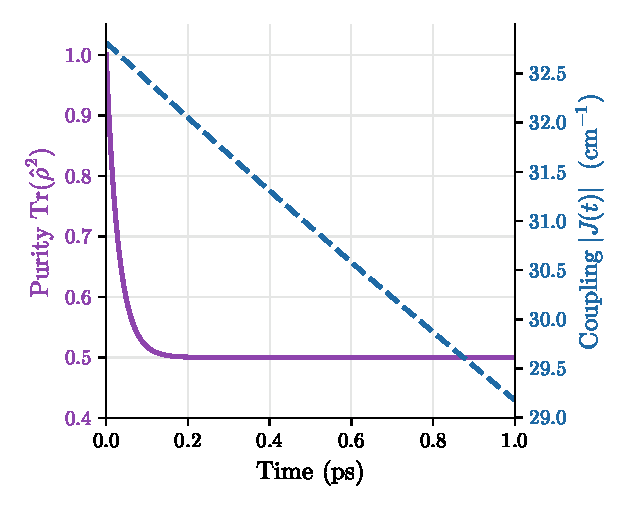
\includegraphics[width=\linewidth]{Fig_Purity_Coupling.pdf}
    \caption{}
    \label{fig:purity_coupling}
  \end{subfigure}\hfill
  \begin{subfigure}[b]{0.32\textwidth}
    \centering
    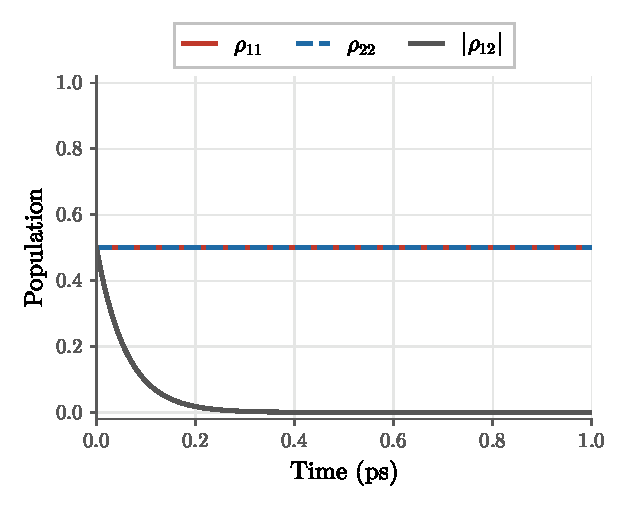
\includegraphics[width=\linewidth]{Fig_ME_Site.pdf}
    \caption{}
    \label{fig:me_site}
  \end{subfigure}\hfill
  \begin{subfigure}[b]{0.32\textwidth}
    \centering
    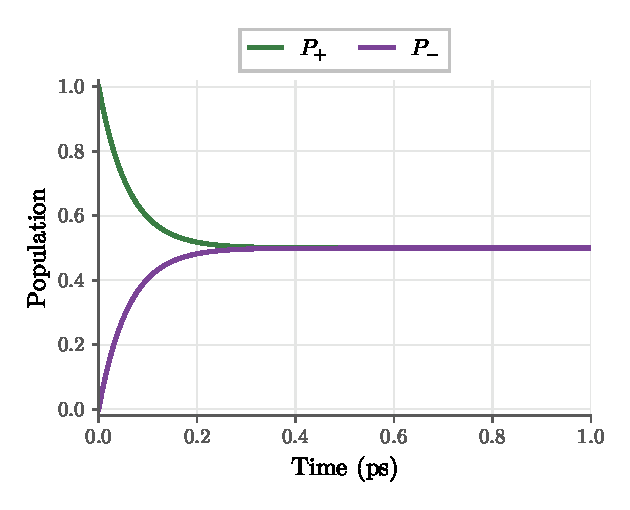
\includegraphics[width=\linewidth]{Fig_ME_Adiabatic.pdf}
    \caption{}
    \label{fig:me_adiabatic}
  \end{subfigure}

  \caption{
  Simulation of excitonic dynamics in the Venus dimer with the local site states $\ket{1}\equiv\ket{e_L g_R}$ and $\ket{2}\equiv\ket{g_L e_R}$: (a) Unified Bloch sphere showing one diffusive stochastic pure-state trajectory (red) and the ensemble-averaged mixed-state path (blue); (b) Site-basis populations and coherence for that SSE trajectory; (c) Adiabatic populations of the symmetric and antisymmetric excitons $\ket{\pm}$ for the same trajectory. (d) Evolution of the purity $\mathrm{Tr}(\hat{\rho}^2)$ and the magnitude of the time-dependent excitonic coupling $|J(t)|$; (e) Ensemble-averaged Master Equation (ME) site-basis populations and coherence; (f) Ensemble-averaged ME adiabatic populations. Time progression: in (a) both paths begin at the chosen symmetric state $\ket{+}$ on the equator, with the individual trajectory (red) executing surface-preserving stochastic excursions and the ensemble average (blue) contracting radially inward toward the maximally mixed centre; in (b-f) time increases from left to right. The rapid sub-$100$\,fs decay of the site-basis coherence $|\rho_{12}|$ is shown explicitly in panels (b) and (e).}
  \label{fig:ExcitonDynamics}
\end{figure*}

To describe the excitonic interactions within the dimer, we restrict our model to the single-exciton manifold, defining the local site basis as $\ket{1}\equiv\ket{e_L \, g_R}$ and $\ket{2}\equiv\ket{g_L \, e_R}$. That restriction deserves justification rather than assertion, because the truncated basis also contains the ground state $\ket{0}\equiv\ket{g_L g_R}$ and the doubly excited state $\ket{3}\equiv\ket{e_L e_R}$, and the former couples to the single-exciton manifold by a matrix element that is not small.

The coupling $\langle 0|\hat V|1\rangle$ is the Coulomb interaction between one chromophore's \emph{transition} density and the other's \emph{permanent} charge density. Because the mature CR2 chromophore is anionic, the partner presents a net $-1\,e$ monopole, so this term falls off as $R^{-2}$ rather than the $R^{-3}$ of the excitonic coupling, and unscreened it is $292~\mathrm{cm^{-1}}$ at the crystallographic separation --- nine times $J$ itself. Three considerations reduce it to a negligible correction. First, the screening is not the optical one. The excitonic coupling connects two transition densities at optical frequency and is correctly screened by $\varepsilon_{\mathrm{opt}}$, whereas $\langle 0|\hat V|1\rangle$ acts against a static charge distribution with which the protein and solvent have fully equilibrated before absorption, so it is screened by the equilibrium response. Second, the intermediate state is the full optical gap away, so the induced correction to the effective coupling is second order, $J_{01}J_{02}/(E_e-E_g)$. Third, the diagonal consequence of that same monopole --- the electrochromic shift it imposes on the partner site energy --- is already contained in the QM/MM site energies, which retain the partner chromophore's RESP charges in the embedding field; only the off-diagonal mixing is at issue here. Numerically, the second-order correction to $J$ is $1.42~\mathrm{cm^{-1}}$ at $\varepsilon_{\mathrm{opt}} = 1.77$, $0.28~\mathrm{cm^{-1}}$ at a pessimistic protein-interior $\varepsilon = 4$, and $0.001~\mathrm{cm^{-1}}$ at the equilibrium $\varepsilon_s = 78$; the ground-state admixture is at most $1.5\times10^{-2}$. Even the most pessimistic of these is below $1\%$ of $J$ and well inside the ensemble spread of $\pm1.55~\mathrm{cm^{-1}}$.

The doubly excited state is further removed. It lies near $2E_e \approx 38\,200~\mathrm{cm^{-1}}$, detuned from the single-exciton block by the entire optical gap, some $580$ times $J$, so its admixture is of order $10^{-3}$ and it does not affect the linear spectrum. It is not, however, irrelevant in general: $\ket{3}$ is the state that makes two-photon absorption a distinct observable and the state from which a dimer can emit two photons, so a description of two-photon or photon-antibunching data requires the full $4\times4$ block even though the $2\times2$ single-exciton treatment is sufficient for the absorption and CD analysed here. This notation restricts the dynamics to the one-photon, single-excitation subspace in which one excitation is shared between the two chromophores. The $\beta$-barrel of Venus has a diameter of $\sim 22$~\AA\ and a closest inter-chromophore approach of 15~\AA\ in the crystal structure of the dimeric Venus fluorescent protein homodimer~\cite{kim2019venusa206}, effectively precluding significant short-range Dexter exchange interactions~\cite{skourtis2016dexter}. We therefore model the electronic coupling $J$ as the Coulomb interaction between the transition densities of the individual monomers \cite{hsu2009}. The electron transition density, $\rho^{g\to e}_m(\mathbf r)$, is obtained by integrating the product of the ground and excited state wavefunctions over the coordinates of $N-1$ electrons in a monomer:
\begin{multline} \label{eq:transition_density}
    \rho^{g\to e}_m(\mathbf{r}) =
    N \int \dots \int d\mathbf{r}_2 \dots d\mathbf{r}_N \\ \Psi_e^*(\mathbf{r}, \mathbf{r}_2, \dots, \mathbf{r}_N) \, \Psi_g(\mathbf{r}, \mathbf{r}_2, \dots, \mathbf{r}_N)
\end{multline}
where $\Psi_g$ and $\Psi_e$ are the many-body electronic wavefunctions for the ground and excited states, respectively ($m=L,\,R$).
The excited-state wavefunction $\Psi_e$ is itself a superposition of configurations obtained by promoting electrons out of the orbitals occupied in the ground-state reference $\Phi_0$ into unoccupied (virtual) orbitals,
\begin{multline} \label{eq:ci_expansion}
    \Psi_e = c_0\,\Phi_0 + \sum_{ia} c_i^{a}\,\Phi_i^{a}
    + \sum_{i<j,\,a<b} c_{ij}^{ab}\,\Phi_{ij}^{ab} \\
    {}+ \sum_{i<j<k,\,a<b<c} c_{ijk}^{abc}\,\Phi_{ijk}^{abc} + \cdots,
\end{multline}
where $i,j,k$ label occupied and $a,b,c$ virtual orbitals: $\Phi_i^{a}$ promotes one electron (a \emph{singly} excited, one-particle/one-hole configuration), $\Phi_{ij}^{ab}$ promotes two at once (a \emph{doubly} excited, ``2p2h'' configuration) and $\Phi_{ijk}^{abc}$ three (\emph{triply} excited, ``3p3h''). This expansion is wavefunction language: configuration-interaction singles retains only the $c_i^{a}$ amplitudes, whereas conventional adiabatic linear-response TDDFT has only poles associated with single Kohn--Sham orbital transitions and therefore cannot represent genuine double-excitation poles \cite{maitra2004double}.

We therefore obtain the correlated site energy and transition density from DLPNO-STEOM-CCSD. STEOM starts from a CCSD-correlated ground state and uses a second similarity transformation built from ionization- and electron-attachment-EOM-CCSD amplitudes before diagonalisation in a compact singles-like space (the construction is summarised in the Methods). It is designed for excited states dominated by one-particle/one-hole character; standard STEOM-CCSD is not an explicit triples method and is not intended for satellite states dominated by double excitations. We calibrate it on the smaller, tractable gas-phase chromophore, where the non-iterative triples correction EOM-CCSD(fT) can be afforded: the STEOM-CCSD wavelength lies close to the triples-corrected result and removes most of the overestimate of bare EOM-CCSD (Table~\ref{tab:ladder}). We use this numerical agreement as an empirical method calibration for the present bright state, not as a claim that STEOM contains full connected triples.

Crucially, while the total electron density is a positive-definite observable representing the probability of finding an electron, the electron transition density implies an off-diagonal matrix element. Since $\int \rho^{g\to e}(\mathbf{r}) d\mathbf{r} = 0$ due to the orthogonality of the ground and excited states, its spatial distribution, characterised by positive and negative phases, indicates the transition's multipolar character. For example, weighting the transition density by the position vector yields the transition dipole moment ($\boldsymbol{\mu} = \int \mathbf{r} \rho^{g \to e}(\mathbf{r}) d\mathbf{r}$), which dictates the far-field optical response. In atomic units, the full TDC is given by the 3D spatial integral
\begin{equation}
    J_{\mathrm{TDC}} \approx \frac{1}{\varepsilon(t)}\iint \frac{\left(\rho^{g\to e}_L(\mathbf r)\right)^*\,\rho^{g\to e}_R(\mathbf r')}{|\mathbf r-\mathbf r'|} \,d\mathbf r\,d\mathbf r'
    \label{eq:J_integral}
\end{equation}
for the relative time-dependent permittivity $\varepsilon(t)$; equivalently, the SI Coulomb prefactor is $1/[4\pi\varepsilon_0\varepsilon(t)]$.
Formally, the electron transition density can be complex, and the conjugate gives the Hermitian coupling matrix element. For the real, non-degenerate molecular states used here, the transition densities and $J$ are real; the sign of $J$ still depends on the arbitrary relative phase chosen for the two isolated-monomer excited states. We use the transition-density-cube (TDC) construction of Krueger et al.~\cite{krueger1998}. The continuous density is discretised in atomic units on a Cartesian grid as $J \approx\frac{1}{\varepsilon(t)}\sum_{i\in L}\sum_{j\in R}\frac{q_i q_j}{|\mathbf r_i-\mathbf r_j|}$, where $q_i=\rho^{g\to e}_L(\mathbf r_i)\,\Delta V$ and $q_j=\rho^{g\to e}_R(\mathbf r_j)\,\Delta V$ are grid-cell transition charges (voxel density times voxel volume), not atom-centred transition charges. For comparison, we also evaluate the far-field PDA, which collapses these densities into two idealised point dipoles $\boldsymbol{\mu}_m$ separated by vector $\mathbf{R}$ given by
\begin{equation} \label{eq:J_PD}
    \resizebox{.98\columnwidth}{!}{$\displaystyle
    J_{\mathrm{PDA}} = \frac{1}{\varepsilon(t)} \left( \frac{\boldsymbol{\mu}_L \cdot \boldsymbol{\mu}_R}{|\mathbf{R}|^3} - \frac{3(\boldsymbol{\mu}_L \cdot \mathbf{R})(\boldsymbol{\mu}_R \cdot \mathbf{R})}{|\mathbf{R}|^5} \right)$}.
\end{equation}

The Coulomb integral is screened by a time-dependent effective permittivity $\varepsilon(t)$ that tracks the solvent response. The aqueous environment relaxes with a Debye time $\tau_D \approx 8.3$\,ps; because this timescale is substantially longer than vertical excitation and the modelled sub-picosecond electronic evolution, the solvent cannot undergo bulk nuclear equilibration over that interval. The permittivity is therefore initially governed by the optical dielectric constant ($\varepsilon_{\rm opt}=1.77$ in the numerical model) and only later approaches the static limit ($\varepsilon_{\rm eq} \approx 78$), as described by
\begin{equation}
    \frac{1}{\varepsilon(t)} = \frac{1}{\varepsilon_{\rm eq}} + \left(\frac{1}{\varepsilon_{\rm opt}} - \frac{1}{\varepsilon_{\rm eq}}\right)e^{-t/\tau_D}.
\end{equation}

Assuming a structurally identical homodimer where the ground to first excited state excitation energies are identical for each monomer ($E_L = E_R = E$), the excited state Hamiltonian in the site basis is
\begin{equation}
    \hat H_{\text{site}}(t)=\begin{pmatrix} E & J(t) \\ J(t) & E \end{pmatrix}.
\end{equation}
Diagonalising $\hat H_{\text{site}}(t)$ yields the adiabatic (exciton) basis, whose eigenstates are the symmetric and antisymmetric combinations $\ket{\pm} = \frac{1}{\sqrt{2}}(\ket{1} \pm \ket{2})$. Their energy separation is the Davydov splitting, $\Delta E(t) = 2|J(t)|$. For non-parallel monomer transition dipoles both exciton states can carry oscillator strength, so we do not identify $\ket{+}$ and $\ket{-}$ as a rigorously bright--dark pair. The dynamics use the symmetric state $\ket{+}$ as an explicit, polarization-selective initial condition and are seeded with the optical-limit coupling at the instant of absorption, $J(0)$. Over several picoseconds, the coupling $J(t)$ relaxes as the solvent environment reorganises from the initial optical dielectric response toward the static equilibrium limit, resulting in a gradual damping of the excitonic interaction. With the numerical value $\varepsilon_{\rm opt}=1.77$, over the plotted first picosecond $1/\varepsilon(t)$ decreases from $0.565$ to $0.502$, so $J(t)$ and the instantaneous splitting $2|J(t)|$ decrease by $11.1\%$. This modest rescaling does not alter the ensemble electron dynamics for this initial condition in the symmetric homodimer model: because $\hat H(t)=E\hat I+J(t)\hat\sigma_x$ and the $\ket{+}$ density operator commutes with $\hat\sigma_x$, replacing $J(t)$ by the frozen value $J(0)$ changes the master-equation site populations, coherence, and $\ket{\pm}$ probabilities only at numerical round-off ($<10^{-12}$). Individual stochastic unravellings change pathwise, as expected, but their ensemble-averaged observables remain identical.

To represent local pure dephasing, we define the master equation (ME) with the rate-normalised Hermitian jump operator $\hat{L} = \sqrt{\gamma/2}\,\hat{\sigma}_z$ in the site basis and the pure-dephasing rate $\gamma = 1/T_2^*$; with this convention $\hat L$ has units of inverse square-root time and the dissipator below damps $\rho_{12}$ at rate $\gamma$. For our simulations, a homogeneous pure-dephasing time of $T_2^* = 60$\,fs was used, the rate at which environmental fluctuations randomise the relative phase of the two site states and damp the off-diagonal coherence $\rho_{12}$, as distinct from the population-relaxation time $T_1$. While the rigid $\beta$-barrel of fluorescent proteins can partially shield chromophores from solvent fluctuations and extend coherence relative to unbound organic dyes \cite{kim2019venusa206}, this conservatively fast $60$\,fs limit was chosen to align with empirical measurements of rapidly decaying electronic quantum coherence in solvated pigment-protein complexes at ambient temperatures \cite{duan2017nature}. {We stress that $T_2^*$ enters as a phenomenological, order-of-magnitude parameter transferred from these analogous systems: no $T_2^*$ has been measured for the Venus dimer, and, importantly, it is deliberately \emph{not} extracted from our classical thermal trajectory. Homogeneous dephasing is governed by a quantum-mechanical energy-gap correlation function and detailed balance. Classical molecular dynamics can provide an approximate correlation function when combined with QM/MM gap calculations and a stated quantum correction, but the present trajectory samples geometry and coupling only, not the required time series of site-energy gaps. What the classical ensemble \emph{does} legitimately supply here is the complementary \emph{inhomogeneous} broadening from the static spread of the coupling over thermally sampled geometries (the $\pm 1.6~\mathrm{cm^{-1}}$ distribution of $J$ in Fig.~\ref{fig:tandem}); site-energy disorder is not sampled in the present $1$\,ns ensemble. Sweeping $T_2^*$ over $20$--$200$\,fs gives coherence-decay times of approximately $0.02$--$0.2$\,ps, all well below the $8.3$\,ps Debye time, so the separation between dephasing and bulk solvent relaxation is robust. Spectral resolution, however, does depend on $T_2^*$: the simple Lorentzian homogeneous FWHM $1/(\pi cT_2^*)$ is $177~\mathrm{cm^{-1}}$ at $60$\,fs, larger than the corrected $2|J|=65.6~\mathrm{cm^{-1}}$; equality occurs only at $T_2^*\approx162$\,fs. Thus the dynamics illustrate post-absorption dephasing and justify optical-limit rather than static dielectric screening at excitation, but do not by themselves establish that the corrected doublet is spectroscopically resolved.} Under this site-local dephasing model, the local site states $\ket{1}$ and $\ket{2}$ form the decoherence-resistant pointer basis. The system's ensemble-averaged density matrix $\hat{\rho}(t)$ in the $\{\ket{1},\ket{2}\}$ basis evolves via the Lindblad equation \cite{manzano2020short}, given by
\begin{equation}
    \frac{d\hat{\rho}}{dt}=-\frac{i}{\hbar}[\hat H_{\text{site}}(t),\hat\rho] + \hat{L} \hat\rho \hat{L} - \frac{1}{2} \{\hat{L}^2, \hat\rho\}\,.
    \label{eq:ME01}
\end{equation}

Building on the Lindblad model, we extend the analysis by simulating individual pure-state trajectories in addition to the ensemble density operator \cite{abrahams2025excitonic}. While the ME provides a deterministic description of the average behaviour of a large ensemble of dimers, it cannot resolve the pathwise fluctuations experienced by a single realisation. To capture these dynamics, we use a stochastic Schrödinger equation (SSE), which describes the evolution of a single pure-state trajectory $|\psi\rangle$ subject to continuous environmental monitoring. The density operator is recovered by taking the stochastic average $\mathbb{E}$ over many trajectories, $\hat{\rho} = \mathbb{E}[|\psi\rangle\langle\psi|]$. Then, the SSE is given by
\begin{multline}
    |d\psi\rangle = \left( -\frac{i}{\hbar}\hat{H}_{\text{site}} - \frac{1}{2}(\hat{L} - \langle \hat{L} \rangle)^2 \right) |\psi\rangle dt \\
    + (\hat{L} - \langle \hat{L} \rangle) |\psi\rangle dW \, ,
\end{multline}
where $dW$ is an It\^{o} Wiener process~\cite{petruccione}.

We visualise an individual pure-state trajectory (\textbf{Figures~\ref{fig:ExcitonDynamics}(b) and (c)}) by mapping the system to the Bloch vector $\mathbf{r} = (\langle\hat\sigma_x\rangle, \langle\hat\sigma_y\rangle, \langle\hat\sigma_z\rangle)$ (\textbf{Figure~\ref{fig:ExcitonDynamics}(a)}), where $\langle\hat\sigma_x\rangle = 2\text{Re}(\rho_{12})$, $\langle\hat\sigma_y\rangle = 2\text{Im}(\rho_{12})$, and $\langle\hat\sigma_z\rangle = \rho_{11} - \rho_{22}$. All the numerical simulations are initialised in the delocalised symmetric state $\ket{+}$, corresponding to a vector on the equator of the Bloch sphere. The diffusive unraveling produces continuous stochastic localisation excursions in the site basis; in the exciton basis these appear as stochastic redistribution between the $\ket{+}$ and $\ket{-}$ components. Each pure-state path remains on the surface of the sphere, as shown in \textbf{Figure~\ref{fig:ExcitonDynamics}(a)}. Conversely, the ensemble-averaged dynamics governed by the ME in Eq.~(\ref{eq:ME01}) describe the rapid, smooth decay of off-diagonal coherence, leading to a statistical mixture over both sites and evolution toward the centre of the Bloch sphere, shown as the solid blue line in \textbf{Figure~\ref{fig:ExcitonDynamics}(a)}.

\section{Computational Methods}

The released quantum-classical workflow is coordinated by \texttt{reproduce\_paper.py}, which integrates the QM/MM electronic-structure calculations (TDDFT, DLPNO-STEOM-CCSD, and the EOM-CCSD/EOM-CCSD(fT) calibration), static GPU-accelerated TDC analysis, and validated numerical archives behind a common configuration. Because the raw 1-ns trajectory and its full-grid $1000$-frame Coulomb calculation are unusually large, that definitive production route is executed by the dedicated \texttt{run\_\allowbreak production\_\allowbreak cr2\_\allowbreak 1000.ps1}, \texttt{extract\_\allowbreak cr2\_\allowbreak transforms.py}, and \texttt{run\_\allowbreak coupling\_\allowbreak production\_\allowbreak cr2\_\allowbreak 1000.ps1} tools; the orchestrator consumes the resulting archive only after checking its frame count and reciprocal-distance unit metadata. Algorithm \ref{alg:pipeline} serves as a concise, reproducible map linking each manuscript quantity to the released routine that produces it, rather than introducing new methodology; readers interested only in the physical results may skip it.

The simulation of the dimeric Venus (PDB: 1MYW \cite{berman2000protein}) proceeded through the following stages.

\begin{enumerate}
    \item \textbf{Structural Preparation and Relaxation:} Geometries for both the isolated monomer and the full interacting dimer were prepared and solvated using PDBFixer \cite{openmm2017} and OpenMM \cite{openmm2017}. Classical energy minimisation of both systems was performed to generate a relaxed AMBER14 \cite{amber14_manual} force-field environment. Within the relaxed monomer, the 29 physical CR2 atoms were then relaxed by a constrained ground-state QM/MM minimisation at $\omega$B97X-D3/6-31G* with the other atoms in the 274-atom QM region frozen and the MM point-charge field present. The frozen $44$-atom electronic-structure geometry combines these gradient-converged CR2 coordinates (plus two rebuilt link hydrogens) with the Tyr203 phenol from the classically minimised monomer (plus one link hydrogen). The relaxed dimer geometry was retained exclusively as the 3D spatial frame for the later coupling analysis. To partition the system for QM/MM embedding it is necessary to sever the protein backbone; to avoid introducing artificial chemical instability, these severed bonds were capped with hydrogen atoms. The $44$ atoms are the complete anionic CR2 chromophore ($29$ atoms), the $\pi$-stacked Tyr203 phenol group only ($12$ atoms: CG, CD1, CD2, CE1, CE2, CZ, OH and five hydrogens), cut at the C$_\gamma$--C$_\beta$ bond so that the tyrosine C$_\beta$ and backbone are excluded, and $3$ link hydrogens capping N1 and C10 of CR2 and C30 of the tyrosine at $1.010$, $1.090$ and $1.090~\text{\AA}$; the stoichiometry is C$_{19}$H$_{18}$N$_3$O$_4$ with net charge $-1$, and retaining the tyrosine C$_\beta$ rather than capping it yields a count of $45$ instead. The region is drawn at three orientations in \textbf{Figure~\ref{fig:qmregion}}.

    \item \textbf{TDDFT reference (ORCA):} As a single-excitation reference, excited-state roots were computed via TDDFT (range-separated hybrid $\omega$B97X-D3/6-311G** \cite{mardirossian2017}, Tamm--Dancoff approximation) in ORCA 6.1 \cite{neese2020orca,neese2022orca} on the \emph{same} $44$-atom QM region and MM point-charge field as the DLPNO-STEOM-CCSD calculation, so that the single-excitation and correlated site energies are compared on an identical structure and embedding.

    \item \textbf{Correlated site energy and transition density (ORCA):} Because the anionic chromophore's site energy is strongly method dependent, the site energy and transition density used for the coupling were computed with DLPNO-STEOM-CCSD \cite{nooijen1997steom,dutta2016dlpno,dutta2018ipeom,dutta2019eaeom,riplinger2013dlpno} as implemented in ORCA 6.1 \cite{neese2020orca,neese2022orca}, using the def2-SVPD basis \cite{weigend2005def2,rappoport2010svpd} with the RIJCOSX approximation, TightSCF/TightPNO thresholds and an automatically constructed auxiliary basis. STEOM-CCSD reaches the excited states through a second similarity transformation of the CCSD Hamiltonian $\bar H = e^{-\hat T}\hat H\,e^{\hat T}$, forming $\tilde H = \{e^{-\hat S}\bar H\,e^{\hat S}\}$ with $\hat S = \hat S^{\mathrm{IP}} + \hat S^{\mathrm{EA}}$ built from ionization- and electron-attachment-EOM-CCSD amplitudes; $\tilde H$ is then diagonalised in a compact singles-like excitation space. Correlation effects enter through the CCSD ground state and the two similarity transformations, but standard STEOM-CCSD does not contain the full connected-triples operator $\hat T_3$ and is intended for roots dominated by single excitations. To keep the correlated calculation tractable while retaining the residue that controls the in-protein shift, Tyr203 was included because its $\pi$--$\pi$ stacking interaction with the conjugated CR2 chromophore directly perturbs the chromophore's electronic environment and site energy. Figure~\ref{fig:qmregion} shows the complete QM structure. The hydrogen-capped, net-$-1$ QM region contains 31 atoms from anionic CR2 (including two link hydrogens) and 13 atoms from the Tyr203 phenol (including one link hydrogen), giving exactly 44 atoms; the rest of the protein and solvent is represented by the MM point-charge field. Root-wise convergence, CIS following, root homing, per-root checks, and the double-excitation filter were enabled to make the active-space construction and reported bright state reproducible. All seven printed S$_1$ natural-transition-orbital pairs (99.046\% total occupation) were combined with their signed singular amplitudes. Voxels assigned by a nearest-QM-atom Voronoi construction to the three artificial link hydrogens were removed, and the cap-masked density was scaled by least-squares projection onto the ORCA right transition moment before applying the relative $10^{-6}$ cutoff. The retained grid preserves the source-frame moment norm to within 0.02\%. Because truncation leaves a small residual transition charge ($-0.00155e$, 0.169\% of the total absolute grid weight), PDA and multipole moments are evaluated about each grid centroid to make them translation invariant. Two independent exact-neutrality constructions change the static TDC by only 1.8\% and leave the conclusion unchanged. This correlated single-point was evaluated at the frozen composite geometry defined above; the complete CR2--Tyr203 $44$-atom cluster was not separately reoptimised. The definitive inter-chromophore coupling is then obtained by evaluating this density over the thermally sampled tandem ensemble (below) rather than from any single geometry.

Figure~\ref{fig:qmregion} gives the atom-resolved chemical structure of the common $44$-atom model used for the embedded and gas-phase electronic-structure comparison.


    \item \textbf{Method calibration (Q-Chem):} STEOM-CCSD was calibrated for this transition on the tractable gas-phase (neutral) chromophore against canonical EOM-CCSD and its non-iterative triples correction EOM-CCSD(fT) \cite{manohar2008ft}, both in Q-Chem \cite{epifanovsky2021qchem} (Table~\ref{tab:ladder}). Agreement with EOM-CCSD(fT) is used here as a numerical calibration; it is not interpreted as formal equivalence to an explicit triples method.

    \item \textbf{Transition Density Coupling (TDC):} The inter-chromophore coupling $J$ was evaluated by reconstructing the full dimeric interaction from the monomeric data. The transition density was duplicated and spatially mapped onto the two chromophore sites of the classically relaxed dimer geometry by a rigid (Kabsch) fit of the shared CR2 atoms, ensuring the STEOM density is placed in the same coordinate frame from which the dimer chains were built; direct numerical integration was then performed across the aligned grids. The production ORCA cube is a $100\times100\times100$ Cartesian grid with spacings $0.155$--$0.172~\text{\AA}$ (voxel volume $4.15\times10^{-3}~\text{\AA}^{3}$). After the link-cap mask, a relative density cutoff of $10^{-6}$ leaves exactly $259{,}277$ signed grid-cell charges per monomer for the Coulomb double sum, which is accumulated on the GPU (Numba-CUDA or PyOpenCL \cite{lam2015numba,klockner2012pycuda}). Because those pair distances are evaluated in \AA, the reciprocal-distance sum is converted to atomic units with $1~\text{\AA}^{-1}=0.529177~a_0^{-1}$ before dielectric screening. We note that such couplings can alternatively be evaluated from atom-centred transition charges fitted to the electrostatic potential (the TrEsp construction) \cite{madjet2006tresp,hsu2009}; the dense-grid integral used here is instead the Krueger TDC construction and additionally supplies the volumetric densities of Figures~\ref{fig:density_combined}--\ref{fig:electron_combined}. As an independent implementation regression, we performed a gas-phase $\omega$B97X-D3/6-311G** calculation on two $54$-atom fragments at a crystal-derived geometry in ORCA: the grid TDC and PDA magnitudes are $6.09$ and $5.36~\mathrm{meV}$, respectively. Numerical results were subsequently screened by the optical dielectric constant ($\varepsilon_{\rm opt}=1.77$ in the numerical model) to account for the sub-picosecond timescale of exciton formation relative to bulk solvent relaxation.
\end{enumerate}

{To sample the room-temperature conformational dynamics that modulate the inter-chromophore geometry and hence $J$, we built the VenusA206 tandem dimer (VenusA206-TD): two Venus $\beta$-barrels covalently joined by the flexible ${\sim}33$-residue inter-domain linker used in the tandem constructs, with the barrels docked at the physiological A206 interface (residues clustered around Ala206, Leu207, Leu221 and Phe223; released tool \texttt{build\_\allowbreak tandem\_\allowbreak dimer.py}). The two CR2 sites received the complete bonded, nonbonded, RESP-charge, exclusion, and $1$--$4$ terms from the production anionic CR2 AMBER topology rather than generic fallback parameters. We then ran $500{,}000$ unrestrained OpenMM NVT steps at $300$\,K with a $2$\,fs timestep ($1$\,ns total), saving the protein and chromophores every $500$ steps to give $1000$ snapshots at $1$\,ps intervals (\texttt{run\_nvt.py}). Periodic imaging was removed by whole-residue lattice translations without coordinate fitting or deformation. For every frame, each copy of the cap-masked STEOM transition density was placed by a rigid fit of the $19$ shared CR2 heavy atoms and the mutual Coulomb integral was accumulated on an RTX 4080 over all $259{,}277^2$ density-point pairs in FP32 (\texttt{coupling\_dcd\_steom.py}); full-grid FP64 checks on frames 1, 500, and 1000 differed by only $0.0031$--$0.0038~\mathrm{cm^{-1}}$. The resulting separation and coupling distributions are reported with the Results (Fig.~\ref{fig:tandem}). Animations of the NVT trajectories are available at \url{https://www.youtube.com/playlist?list=PLbopStXxFpaQ}.}

\begin{algorithm*}[t]
\caption{Quantum-Classical Hybrid Excitonic Coupling Pipeline \\(\texttt{reproduce\_paper.py})}
\label{alg:pipeline}
\footnotesize
\begin{algorithmic}[1]
\Procedure{PipelineMain}{}
    \State \Call{Stage1\_ClassicalSetup}{}
    \State \Call{Stage2\_TDDFT}{}      \Comment{ORCA: single-excitation reference}
    \State \Call{Stage3\_STEOM}{}      \Comment{ORCA: correlated site energy + density}
    \If{validation requested}          \Comment{Stage 4 is optional}
        \State \Call{Stage4\_Calibrate}{} \Comment{Q-Chem: EOM-CCSD/EOM-CCSD(fT)}
    \EndIf
    \State \Call{Stage5\_TDC}{}         \Comment{static and thermal-ensemble coupling}
\EndProcedure

\vspace{0.05cm}
\Procedure{Stage1\_ClassicalSetup}{}
    \State Initialise system with PDBFixer (add missing atoms/hydrogens)
    \State Load AMBER14 XML forcefield parameters
    \State Solvate both dimer and monomer systems
    \State Relax both solvated geometries via OpenMM classical minimisation with explicit-solvent electrostatics (PME when periodic)
    \State Partition system into QM and MM regions (link-atom boundary)
    \State Evaluate formal charges via CCD CIF parsing
    \State Extract MM point charges, excluding charges within $1.8$~\AA{} of the QM boundary and preserving net charge
    \State Relax the physical CR2 atoms by constrained ground-state QM/MM minimisation
    \State Assemble the frozen $44$-atom CR2 + Tyr203 composite geometry and link atoms
    \State Export monomer QM region coordinates as a \texttt{.xyz} file
\EndProcedure

\vspace{0.05cm}
\Procedure{Stage2\_TDDFT}{}
    \State Load the $44$-atom QM region and its MM point-charge field (shared with Stage 3)
    \State Configure ORCA TDDFT ($\omega$B97X-D3/6-311G**, Tamm--Dancoff, point-charge embedding)
    \State Execute TDDFT energy calculation
    \State Parse excited-state roots and select the bright state by highest oscillator strength
    \State Reconstruct the transition density from natural transition orbitals (method-consistency coupling check)
\EndProcedure

\vspace{0.05cm}
\Procedure{Stage3\_STEOM}{}
    \State Build the reduced (CR2 + Tyr203) QM region with MM point-charge field
    \State Run ORCA DLPNO-STEOM-CCSD (def2-SVPD, RIJCOSX, TightPNO)
    \State Verify convergence and deterministic active space; parse bright state
    \State Reconstruct $\rho^{g\to e}$ from natural transition orbitals; scale to the ORCA right transition moment
\EndProcedure

\vspace{0.05cm}
\Procedure{Stage4\_Calibrate}{} \Comment{optional}
    \State Run Q-Chem EOM-CCSD and EOM-CCSD(fT) on the gas-phase chromophore
    \State Compare STEOM numerically with the triples-corrected benchmark
\EndProcedure

\vspace{0.05cm}
\Procedure{Stage5\_TDC}{}
    \State Load the relaxed dimer frame and the STEOM (or TDDFT) transition density
    \State Rigid-fit (Kabsch) the density onto each chromophore site $L,R$
    \State \Call{CalculateCouplingGPU}{Site L, Site R} at the minimised geometry
    \State Repeat over the tandem-dimer NVT ensemble for the distribution
\EndProcedure

\vspace{0.05cm}
\Procedure{CalculateCouplingGPU}{$\mathbf{r}_L, q_L, \mathbf{r}_R, q_R$}
    \State Initialise Numba CUDA or PyOpenCL context
    \State Initialise $J = 0$
    \For{each grid point $i$ in Site A accumulate:}
        \State $J \gets J + \sum_j \frac{q_{L,i} \cdot q_{R,j}}{|\mathbf{r}_{L,i} - \mathbf{r}_{R,j}|}$
    \EndFor
    \State Convert the inverse-\AA{} sum with $1~\text{\AA}^{-1}=0.529177~a_0^{-1}$
    \State Apply optical dielectric screening factor ($\varepsilon_{\mathrm{opt}}$)
    \State \Return Excitonic Coupling $J$
\EndProcedure
\end{algorithmic}
\end{algorithm*}

\clearpage

\begin{figure*}[t]
  \centering
  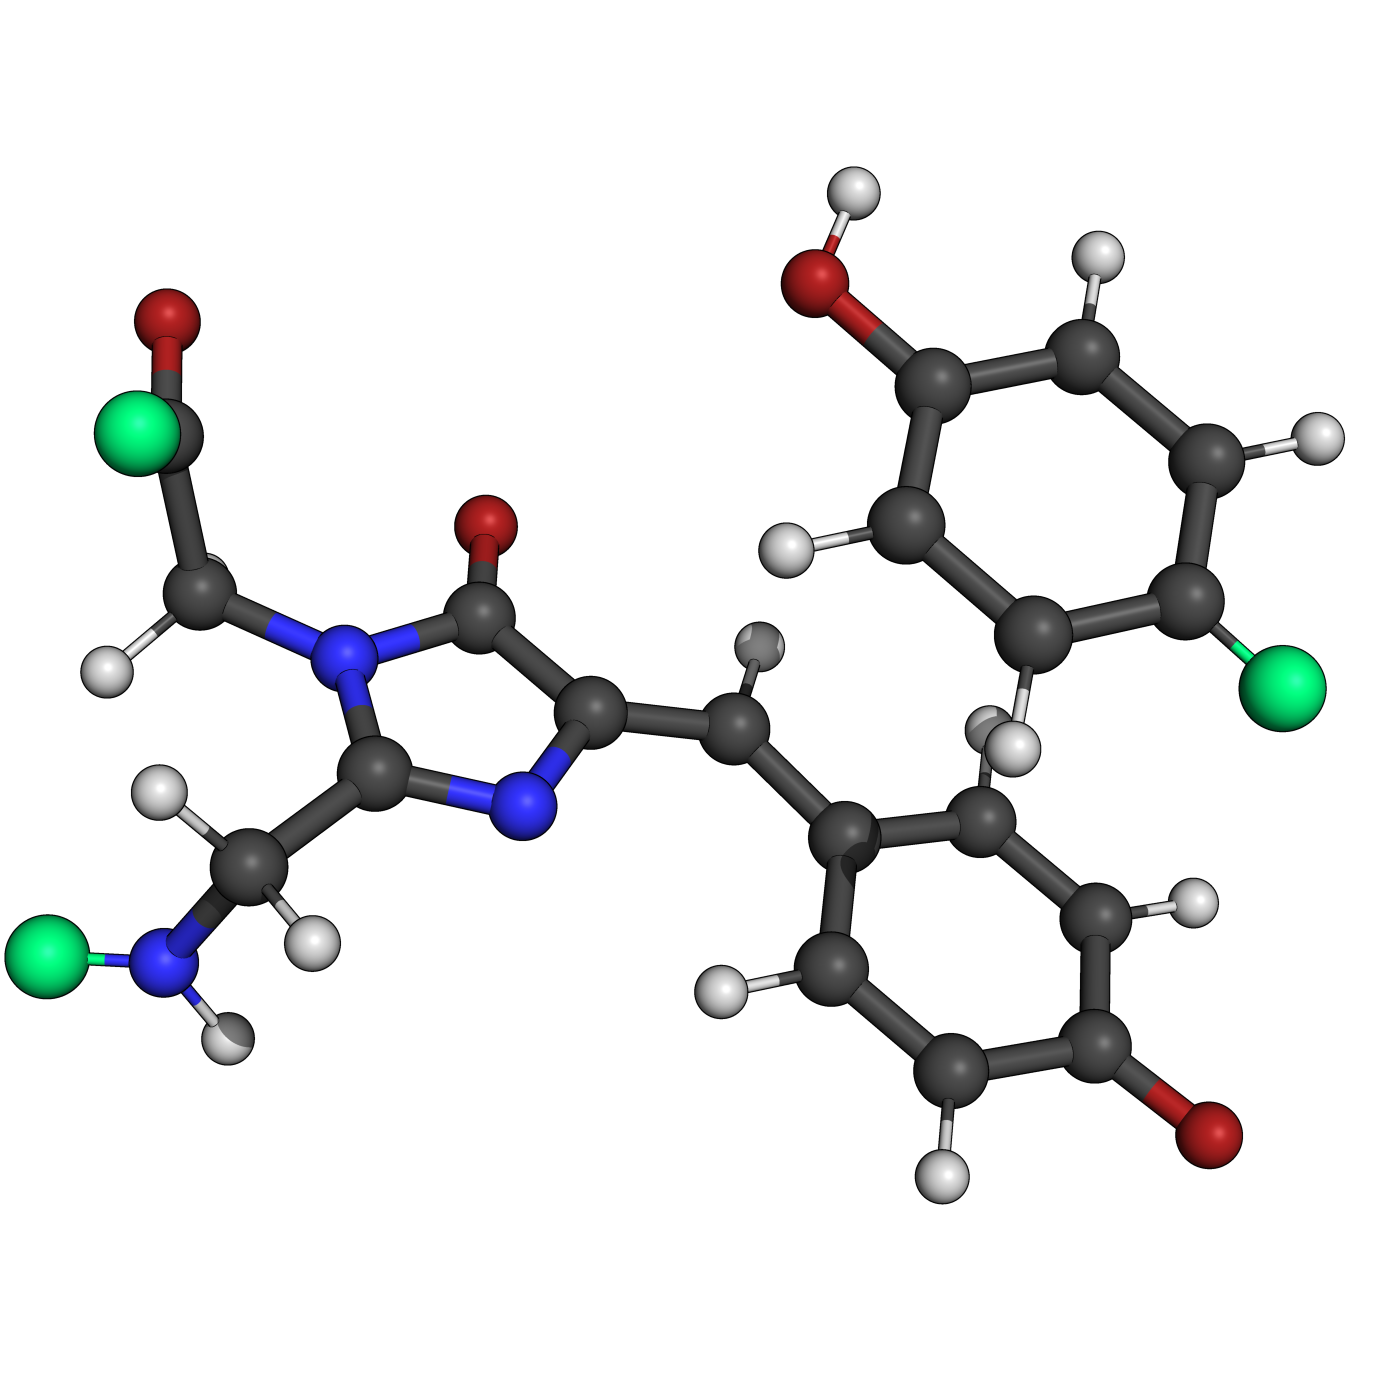
\includegraphics[width=0.31\textwidth]{FigS1_qmregion_a.png}\hfill
  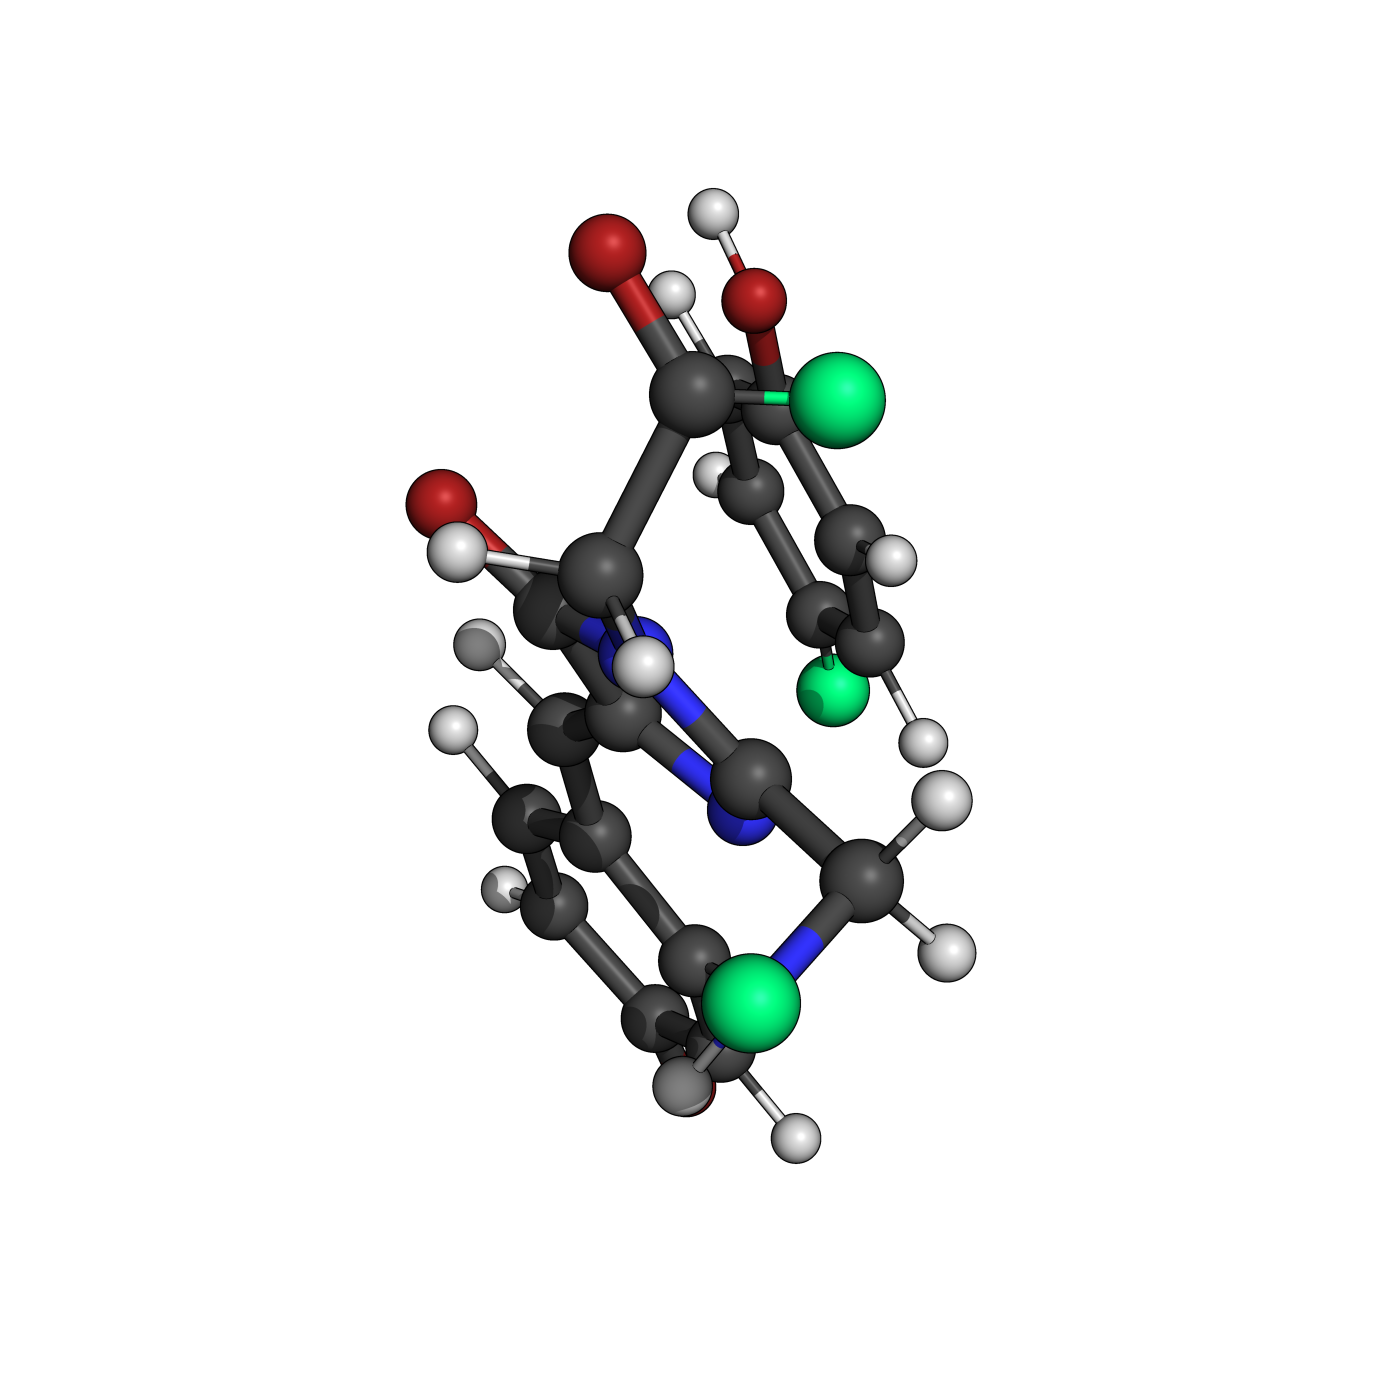
\includegraphics[width=0.31\textwidth]{FigS1_qmregion_b.png}\hfill
  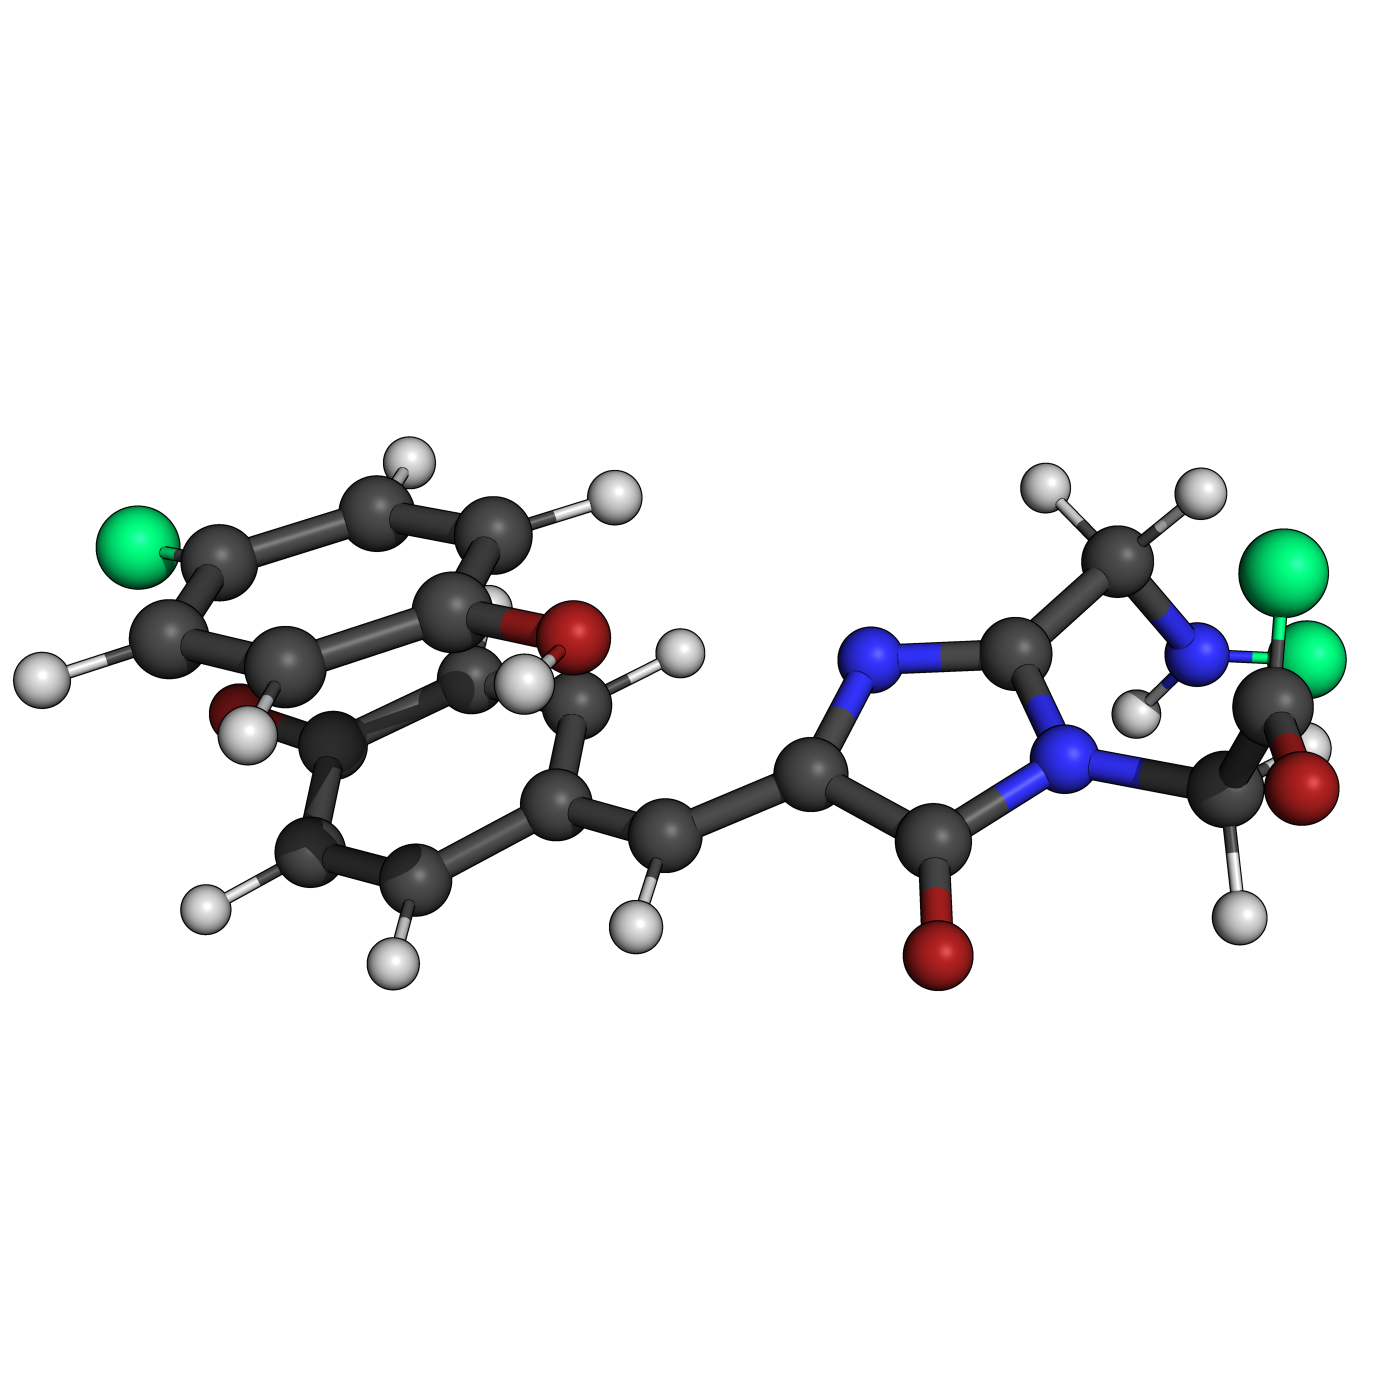
\includegraphics[width=0.31\textwidth]{FigS1_qmregion_c.png}
  \caption{The $44$-atom QM region used for every electronic-structure calculation, drawn from the production geometry at three orientations. Carbon grey, oxygen red, nitrogen blue, hydrogen white; the three link hydrogens are green and enlarged. The anionic CR2 chromophore ($29$ atoms) comprises the imidazolinone at centre and the phenolate ring at lower right; the $\pi$-stacked Tyr203 phenol ($12$ atoms, upper right) retains its hydroxyl. The cut is made at the tyrosine C$_\gamma$--C$_\beta$ bond, and retaining that C$_\beta$ rather than capping it is what yields a count of $45$ atoms. Net charge $-1$, stoichiometry C$_{19}$H$_{18}$N$_3$O$_4$.}
  \label{fig:qmregion}
\end{figure*}

\section{Results and Discussion}

Among the computed visible roots, the chromophore possesses one dominant bright excitation: TDDFT/TDA ($\omega$B97X-D3, computed on the same $44$-atom QM region and point-charge field as the correlated calculation) returns a bright $\pi\pi^{*}$ root ($f=1.033$) at $360.9~\mathrm{nm}$, roughly $154~\mathrm{nm}$ to the blue of experiment. We therefore adopt the correlated wavefunction result as the site energy: the converged DLPNO-STEOM-CCSD electric-dipole spectrum (ORCA \cite{neese2020orca,neese2022orca,nooijen1997steom,dutta2018ipeom,dutta2019eaeom,dutta2016dlpno}) places the in-protein bright state at $523.90~\mathrm{nm}$ ($f=0.885$), in good agreement with the experimental absorption maximum near $515~\mathrm{nm}$ (Table~\ref{tab:roots}). This choice is calibrated on the tractable gas-phase (neutral) chromophore, where a non-iterative triples correction redshifts bare EOM-CCSD from $333.29$ to $376.85~\mathrm{nm}$, close to the STEOM value of $371.21~\mathrm{nm}$ (Table~\ref{tab:ladder}) \cite{manohar2008ft,epifanovsky2021qchem}. To physically characterise the transition, the STEOM electron transition density ($\rho^{g\to e}$) and the ground-to-excited state electron density difference ($\rho^{e} - \rho^{g}$) were mapped onto the dimer frame (\textbf{Figure~\ref{fig:density_combined}} and \textbf{Figure~\ref{fig:electron_combined}}, respectively).

\begin{table}[H]
\centering
\caption{Photon wavelength and oscillator strength of the vertical bright $\pi\pi^{*}$ excitation of the anionic Venus chromophore in the same frozen $44$-atom QM geometry, with the protein/solvent MM point-charge embedding (QM/MM) and after removal of all point charges (gas phase). TDDFT yields a dominant bright $\pi\pi^{*}$ root but blueshifts it; STEOM-CCSD, adopted here as the method of record, agrees with the measured absorption in the embedded model.}
\label{tab:roots}
{\small\setlength{\tabcolsep}{3pt}
\resizebox{\columnwidth}{!}{%
\begin{tabular}{lcccc}
\toprule
& \multicolumn{2}{c}{QM/MM} & \multicolumn{2}{c}{Gas phase} \\
\cmidrule(lr){2-3}\cmidrule(lr){4-5}
Method & $\lambda$ (nm) & $f$ & $\lambda$ (nm) & $f$ \\
\midrule
TDDFT, $\omega$B97X-D3      & 360.9 & 1.033 & 366.0 & 1.262 \\
DLPNO-STEOM-CCSD            & 523.90 & 0.885 & \textit{not defined}\footnotemark[1] & -- \\
Experiment (absorption)     & 514.46 & n/a   & -- & -- \\
\bottomrule
\end{tabular}}}
\footnotetext[1]{The gas-phase coupled-cluster entry is left undefined rather than tabulated. Removing the point-charge field leaves an isolated anion whose electron-attached states are unbound in a diffuse basis, and the EA-EOM step of the STEOM transformation, which uses that sector to dress the excitation, does not converge: the Davidson iterations return complex eigenvalues. The failure is physical rather than technical, and a gas-phase reference for an \emph{anionic} chromophore is therefore not simply the embedded calculation with the charges deleted. The TDDFT row is unaffected because TDA-TDDFT has no electron-attachment sector.}
\end{table}

\begin{table*}[t]
\centering
\caption{Method calibration on the gas-phase (neutral) chromophore, def2-SVP. Bare EOM-CCSD predicts the excitation at too short a wavelength; the non-iterative triples correction EOM-CCSD(fT) redshifts it from $333.29$ to $376.85~\mathrm{nm}$ (a shift of $43.56~\mathrm{nm}$), close to the DLPNO-STEOM-CCSD value of $371.21~\mathrm{nm}$. This numerical agreement supports use of STEOM-CCSD for the present predominantly singly excited bright state; it does not imply that standard STEOM-CCSD is an explicit triples treatment.}
\label{tab:ladder}
\begin{tabular}{lcc}
\toprule
Method & $\lambda$ (nm) & $f$ \\
\midrule
TDDFT, CAM-B3LYP          & 366.9  & 0.801 \\
TDDFT, $\omega$B97X-D3    & 361.3  & 0.829 \\
EOM-CCSD (bare)           & 333.29 & --- \\
EOM-CCSD(fT) (+triples)   & 376.85 & --- \\
DLPNO-STEOM-CCSD          & 371.21 & --- \\
\bottomrule
\end{tabular}
\end{table*}

\begin{figure*}[t]
  \centering
  \begin{subfigure}[b]{0.48\textwidth}
    \centering
    
\includegraphics[width=\linewidth]{steom_transition_dimer.png}
    \caption{}
    \label{fig:density_dimer}
  \end{subfigure}\hfill
  \begin{subfigure}[b]{0.48\textwidth}
    \centering
    
\includegraphics[width=\linewidth]{steom_transition_qm.png}
    \caption{}
    \label{fig:density_qm}
  \end{subfigure}
  \caption{Visualisation of the monomeric electron transition density $\rho^{g\to e}_m(\mathbf r)$ in Eq.~(\ref{eq:transition_density}) between the ground and bright excited state in Table \ref{tab:roots}. The red and blue isosurfaces represent its positive and negative phases, rigidly mapped onto both chromophore sites of the dimer frame using PyMOL structural alignment; this placement is not a separate dimer excited-state calculation. (a) The full dimer system partitioned into QM and MM domains. The MM embedding environment, treated as point charges, is rendered as a protein backbone with a rainbow colourmap to give a sense of depth perception. (b) A detailed view of the $44$-atom STEOM QM region (indicated with sticks and spheres) on the right monomer, comprising the deprotonated CR2 chromophore and the $\pi$-stacked Tyr203 phenol on which the correlated transition density is evaluated. PyMOL \cite{delano2002pymol} generation scripts are available on GitHub.}
  \label{fig:density_combined}
\end{figure*}

The electron transition density in \textbf{Figure~\ref{fig:density_combined}}, which serves as the fundamental quantity for evaluating the Coulombic integral in Eq.~(\ref{eq:J_integral}), exhibits a complex multipolar spatial distribution in 3D that extends across the entire chromophore and adjacent residues. Note that the red and blue isosurfaces in \textbf{Figure~\ref{fig:density_combined}(b)} do not represent static charge gain or loss, but rather the signed lobes of the transition density. Their relative positions and signs on the two chromophores determine the long-range Coulomb integral $J_{\text{TDC}}$; no inter-chromophore density overlap is required. Concurrently, the electron density difference in \textbf{Figure~\ref{fig:electron_combined}(b)} shows the ground-to-excited-state redistribution involving the deprotonated phenolic oxygen and the rest of the conjugated CR2 chromophore without assigning that static difference to a time-resolved charge-transfer pathway.

The production cap-masked STEOM transition density was then mapped onto both sites of the dimer frame (chromophore centroid separation $25.2~\text{\AA}$; inter-dipole angle $103.7^{\circ}$). This computed geometry is consistent with the two-photon polarization ratio measured for the Venus dimer, which independently constrains the relative orientation of the two chromophore transition dipoles \cite{cusick2026polarization}. At this geometry, the full transition-density coupling modestly exceeds the far-field point-dipole approximation:

{\sloppy\setlength{\leftmargini}{1em}
\begin{itemize}
    \item \textbf{Transition-Density Coupling:} $J_{\text{TDC}} = 30.5~\mathrm{cm^{-1}}$,
    \item \textbf{Point-Dipole Approximation:} $J_{\text{PDA}} = 24.8~\mathrm{cm^{-1}}$,
    \item \textbf{Near-field correction:} $J_{\text{TDC}}/J_{\text{PDA}} = 1.23$.
\end{itemize}}

\noindent For comparison, evaluating the same TDC pipeline on the TDDFT transition density of the identical transition (from the same $44$-atom calculation) gives $J_{\text{TDC}} = 22.1~\mathrm{cm^{-1}}$ versus $J_{\text{PDA}} = 18.0~\mathrm{cm^{-1}}$ ($1.23\times$). The size of the distributed-density correction is therefore method-consistent, while the STEOM density couples ${\sim}1.38$ times more strongly than TDDFT at fixed geometry.

\begin{figure*}[t]
  \centering
  \begin{subfigure}[b]{0.48\textwidth}
    \centering
    
\includegraphics[width=\linewidth]{steom_difference_dimer.png}
    \caption{}
    \label{fig:electron_dimer}
  \end{subfigure}\hfill
  \begin{subfigure}[b]{0.48\textwidth}
    \centering
    
\includegraphics[width=\linewidth]{steom_difference_qm.png}
    \caption{}
    \label{fig:electron_qm}
  \end{subfigure}
  \caption{Visualisation of the monomeric STEOM electron density difference ($\rho^{e} - \rho^{g}$) between the ground and bright excited state in Table \ref{tab:roots}, rigidly mapped onto both chromophore sites of the dimer frame. The green and violet isosurfaces represent electron gain and loss, respectively; this placement is a visualisation of the two-site model, not a separate dimer excited-state calculation. (a) The dimer frame illustrating the QM/MM partitioning, with the MM backbone rendered in the rainbow colourmap to give a sense of depth perception. (b) A detailed view of the $44$-atom STEOM QM region on the right monomer, comprising the deprotonated CR2 chromophore and the $\pi$-stacked Tyr203 phenol. The detailed PyMOL \cite{delano2002pymol} codes are available on GitHub.}
  \label{fig:electron_combined}
\end{figure*}

The comparison between the TDC calculation and the far-field point-dipole estimate quantifies a modest near-field correction. At the $25.2~\text{\AA}$ chromophore-centroid separation, the spatially extended STEOM density raises the Coulomb coupling by $23\%$ relative to the PDA; the analogous TDDFT correction is $23\%$. A separate method-matched gas-phase ORCA calculation on a crystal-geometry model gives coupling magnitudes $|J_{\text{TDC}}|=6.09~\mathrm{meV}$ and $|J_{\text{PDA}}|=5.36~\mathrm{meV}$ and supports the corrected implementation. The transition densities remain well beyond the range of significant Dexter exchange \cite{skourtis2016dexter}.

To identify the origin of this correction, we decomposed the coupling into a primitive Cartesian multipole series about each chromophore centroid (companion analysis \texttt{multipole\_analysis.py}, evaluated on the production cap-masked transition density of the bright $\pi\pi^{*}$ state), evaluating the transition dipole, quadrupole and octupole moments and the corresponding inter-site interaction terms (dipole--dipole, dipole--quadrupole, quadrupole--dipole, dipole--octupole, quadrupole--quadrupole, octupole--dipole). The dipole--dipole term reproduces $J_{\text{PDA}}$ exactly by construction and accounts for $81.5\%$ of the full $J_{\text{TDC}}$; adding the dipole--quadrupole terms gives $94.7\%$, including quadrupole--quadrupole gives $95.2\%$, and adding the dipole--octupole terms gives $97.6\%$. Thus, the leading multipoles explain almost all of the finite-density correction, with the remaining $2.4\%$ arising from higher orders. The implementation is independently validated by a self-test that reconstructs an exact brute-force coupling between two compact, well-separated model densities to better than $0.1\%$.

Because protein conformational dynamics modulate the inter-chromophore geometry and hence $J$, we characterised the coupling over a room-temperature trajectory of the actual VenusA206 tandem-dimer construct (see Methods, \textbf{Figure~\ref{fig:tandem}}). The covalently tethered tandem holds the A206 interface docked for the full $1~\mathrm{ns}$: the chromophore separation is $24.69 \pm 0.32~\text{\AA}$ (range $23.72$--$26.08~\text{\AA}$), and the full-grid transition-density coupling is $J = 32.8 \pm 1.6~\mathrm{cm^{-1}}$ (sample standard deviation; splitting $2|J| = 65.6 \pm 3.1~\mathrm{cm^{-1}}$). The corresponding ensemble point-dipole result is $27.6 \pm 1.3~\mathrm{cm^{-1}}$, so the distributed-density calculation is larger by a factor of $1.19$. The covalent linker therefore sustains the docked geometry and a stable, intermediate-regime Coulomb coupling throughout the dynamics.

\begin{figure*}[t]
  \centering
  \begin{subfigure}[b]{0.32\textwidth}
    \centering
    
\includegraphics[width=\linewidth]{Fig_Tandem_Separation.pdf}
    \caption{}
    \label{fig:tandem_sep}
  \end{subfigure}\hfill
  \begin{subfigure}[b]{0.32\textwidth}
    \centering
    \includegraphics[width=\linewidth]{Fig_Detuning_Histogram.pdf}
    \caption{}
    \label{fig:tandem_detuning}
  \end{subfigure}\hfill
  \begin{subfigure}[b]{0.32\textwidth}
    \centering
    
\includegraphics[width=\linewidth]{Fig_Tandem_Histogram.pdf}
    \caption{}
    \label{fig:tandem_hist}
  \end{subfigure}

  \caption{Dynamics of the VenusA206 tandem dimer ($1000$ frames saved every $1$\,ps over a $1$\,ns, $300$\,K unrestrained NVT trajectory; \texttt{run\_nvt.py}, \texttt{coupling\_dcd\_steom.py}). The two anionic CR2 residues use the production AMBER parameters, and every snapshot is evaluated with the complete cap-masked STEOM transition density ($259{,}277\times259{,}277$ mutual Coulomb sum, GPU, $\varepsilon_{\rm opt}=1.77$). (a) Chromophore-centroid separation versus time, $24.69\pm0.32~\text{\AA}$ (mean dashed; shading is one sample standard deviation). (b) Distribution of the QM/MM TDDFT site-energy difference $\Delta = E_A - E_B$ over the ensemble ($n=95$; $\langle|\Delta|\rangle = 576~\mathrm{cm^{-1}}$, median $557~\mathrm{cm^{-1}}$), with $\pm2|J|$ marked by the dashed red lines: only $7$ frames ($7.4\%$) fall inside $|\Delta| < 2|J|$, so the two chromophores are almost never near-degenerate. (c) Distribution of all $1000$ values; the spread is the sample standard deviation, not the uncertainty in the mean.}
  \label{fig:tandem}
\end{figure*}

\newpage
Nguyen et al.\ analysed the $\mathrm{dVenus\mbox{-}TDX}-\mathrm{dVenus\mbox{-}TD}$ difference-molar-ellipticity spectrum with three Lorentzians \cite{nguyen2025anomalous}. Their constrained sensitivity fit (Table~S3) places the excitonic pair at $514.07$ and $521.07~\mathrm{nm}$, giving $U=130.79~\mathrm{cm^{-1}}$ and $2U=261.58~\mathrm{cm^{-1}}$, with a third band at $481.37~\mathrm{nm}$; the unconstrained fit shown in their main Fig.~4(d) instead gives $511.8$ and $521.7~\mathrm{nm}$, or $U\approx185.4~\mathrm{cm^{-1}}$. These are alternative fit conventions rather than the endpoints of a statistical confidence interval. Our corrected ensemble value, $J=32.8~\mathrm{cm^{-1}}$ ($2|J|=65.6~\mathrm{cm^{-1}}$), is about a factor of four below the constrained $U$ value. That factor of four is not a failure of the coupling calculation but a consequence of the degeneracy assumed in the spectroscopic analysis. Both the constrained fit and the earlier Davydov reading place the two components symmetrically about the monomer energy, which is the degenerate-dimer prediction; the detuning never enters. QM/MM site energies on the same construct show that the two chromophores are not isoenergetic, with $\langle|\Delta|\rangle$ of several hundred $\mathrm{cm^{-1}}$, an order of magnitude above $2|J|=65.6~\mathrm{cm^{-1}}$. For a detuned pair the exciton gap is $\Omega=\sqrt{\Delta^{2}+4J^{2}}$, and the rotational strength of each band carries a factor $\sin2\theta=2|J|/\Omega$, so the couplet \emph{separation} reports $\Omega$ while only the couplet \emph{amplitude} reports $J$. Taking $J=32.8$ and $|\Delta|=550~\mathrm{cm^{-1}}$ gives $\Omega=553.9~\mathrm{cm^{-1}}$, or $14.75~\mathrm{nm}$ at $516~\mathrm{nm}$, against the $14.6\pm0.3~\mathrm{nm}$ splitting reported by Kim et al.\ \cite{kim2019venusa206}, with no adjustable parameter, and an amplitude suppressed by $2|J|/\Omega=0.12$ relative to a degenerate pair. Reading the same splitting as $2|J|$ instead requires $J=274~\mathrm{cm^{-1}}$, which at the crystallographic $25.4~\text{\AA}$ separation would demand a transition dipole near $29~\mathrm{D}$ or a separation near $10~\text{\AA}$, neither of which is available to two $\beta$-barrels of diameter $\geq22~\text{\AA}$. The conclusion is supported independently: a two-photon polarisation-ratio analysis of dVenus-TD places the coupling at $32$--$40~\mathrm{cm^{-1}}$ with an H--J splitting of $60$--$90~\mathrm{cm^{-1}}$ \cite{cusick2026twophoton}, bracketing the values computed here.

\clearpage

\begin{figure*}[t]
  \centering
  \begin{subfigure}[b]{0.32\textwidth}
    \centering
    
\includegraphics[width=\linewidth]{frame_deloc/Fig_Bloch_Grid.pdf}
    \caption{}
    \label{fig:fdeloc_a}
  \end{subfigure}\hfill
  \begin{subfigure}[b]{0.32\textwidth}
    \centering
    
\includegraphics[width=\linewidth]{frame_deloc/Fig_SSE_Site.pdf}
    \caption{}
    \label{fig:fdeloc_b}
  \end{subfigure}\hfill
  \begin{subfigure}[b]{0.32\textwidth}
    \centering
    
\includegraphics[width=\linewidth]{frame_deloc/Fig_SSE_Adiabatic.pdf}
    \caption{}
    \label{fig:fdeloc_c}
  \end{subfigure}

  \vspace{0.25cm}

  \begin{subfigure}[b]{0.32\textwidth}
    \centering
    
\includegraphics[width=\linewidth]{frame_deloc/Fig_Purity_Coupling.pdf}
    \caption{}
    \label{fig:fdeloc_d}
  \end{subfigure}\hfill
  \begin{subfigure}[b]{0.32\textwidth}
    \centering
    
\includegraphics[width=\linewidth]{frame_deloc/Fig_ME_Site.pdf}
    \caption{}
    \label{fig:fdeloc_e}
  \end{subfigure}\hfill
  \begin{subfigure}[b]{0.32\textwidth}
    \centering
    
\includegraphics[width=\linewidth]{frame_deloc/Fig_ME_Adiabatic.pdf}
    \caption{}
    \label{fig:fdeloc_f}
  \end{subfigure}

  \vspace{0.25cm}

  \vspace{0.35cm}

  \begin{subfigure}[b]{0.32\textwidth}
    \centering
    
\includegraphics[width=\linewidth]{frame_loc/Fig_Bloch_Grid.pdf}
    \caption{}
    \label{fig:floc_g}
  \end{subfigure}\hfill
  \begin{subfigure}[b]{0.32\textwidth}
    \centering
    
\includegraphics[width=\linewidth]{frame_loc/Fig_SSE_Site.pdf}
    \caption{}
    \label{fig:floc_h}
  \end{subfigure}\hfill
  \begin{subfigure}[b]{0.32\textwidth}
    \centering
    
\includegraphics[width=\linewidth]{frame_loc/Fig_SSE_Adiabatic.pdf}
    \caption{}
    \label{fig:floc_i}
  \end{subfigure}

  \vspace{0.25cm}

  \begin{subfigure}[b]{0.32\textwidth}
    \centering
    
\includegraphics[width=\linewidth]{frame_loc/Fig_Purity_Coupling.pdf}
    \caption{}
    \label{fig:floc_j}
  \end{subfigure}\hfill
  \begin{subfigure}[b]{0.32\textwidth}
    \centering
    
\includegraphics[width=\linewidth]{frame_loc/Fig_ME_Site.pdf}
    \caption{}
    \label{fig:floc_k}
  \end{subfigure}\hfill
  \begin{subfigure}[b]{0.32\textwidth}
    \centering
    
\includegraphics[width=\linewidth]{frame_loc/Fig_ME_Adiabatic.pdf}
    \caption{}
    \label{fig:floc_l}
  \end{subfigure}

  \vspace{0.25cm}

  \caption{The same six quantities as Figure~\ref{fig:ExcitonDynamics}, produced by the same generator with only the two site energies changed, evaluated on the extreme members of the site-energy ensemble rather than at its mean. Panels (a)--(f), frame $465$: $\Delta = +12.9~\mathrm{cm^{-1}}$, the smallest detuning sampled, giving $\Omega = 66.9~\mathrm{cm^{-1}}$, mixing $2|J|/\Omega = 0.981$ and $40.4\%$ of the bright eigenstate on the minor site. Panels (g)--(l), frame $1005$: $\Delta = -1825~\mathrm{cm^{-1}}$, the largest sampled, giving $\Omega = 1826~\mathrm{cm^{-1}}$, mixing $0.036$ and $0.03\%$ on the minor site. Panel order matches Figure~\ref{fig:ExcitonDynamics} in both blocks: Bloch sphere, SSE site basis, SSE adiabatic basis, purity with $|J(t)|$, ME site basis, ME adiabatic basis. In the near-degenerate frame the sites exchange population completely and the Bloch vector sweeps the equator, which is what a delocalised exciton picture presumes; in the detuned frame the populations barely move, the adiabatic states are the site states, and the Bloch vector stays near a pole. Only $7$ of $95$ frames ($7.4\%$) have $|\Delta| < 2|J|$, so the lower block is the typical case.}
  \label{fig:framedynamics}
\end{figure*}

Because the detuning varies by two orders of magnitude across the ensemble, an averaged mixing conceals the physics, and we therefore propagate the two extreme members explicitly (\textbf{Figure~\ref{fig:framedynamics}}). In the near-degenerate frame the two sites exchange population completely and a large site-basis coherence survives for tens of femtoseconds, which is the behaviour a delocalised exciton picture presumes. In the maximally detuned frame the population barely moves, the coherence is an order of magnitude smaller, and the eigenstates are essentially the site states. Since the ensemble average of a nonlinear function is not the function of the average, and the median detuning is several hundred $\mathrm{cm^{-1}}$, the typical dynamics resembles the detuned frame. A coherence claim supported only by the near-degenerate case is therefore a statement about a small tail of the conformational ensemble rather than about the dimer.

\section{Conclusions}

We have characterised the excitonic coupling and energy-transfer dynamics in a Venus dimer using a hybrid QM/MM transition-density approach in an open-quantum-system model. Using a correlated (DLPNO-STEOM-CCSD) site energy and transition density (calibrated against a non-iterative triples-corrected benchmark) and simulating the actual VenusA206 tandem-dimer construct, we find that the covalent inter-domain linker holds the A206 interface docked throughout a nanosecond of dynamics, with $J=32.8\pm1.6~\mathrm{cm^{-1}}$ across $1000$ snapshots and a Davydov splitting of $65.6\pm3.1~\mathrm{cm^{-1}}$ within the broad intermediate excitonic regime. Integrating the distributed transition densities raises the coupling by $19\%$ relative to the ensemble PDA value of $27.6\pm1.3~\mathrm{cm^{-1}}$. The unit-corrected TDC implementation is independently validated against a method-matched gas-phase ORCA control and against an independent referee calculation. The resulting coupling is about fourfold below the constrained CD-derived value, and that factor is accounted for by the site-energy detuning: because $\Omega=\sqrt{\Delta^{2}+4J^{2}}$ with $|\Delta|\gg2|J|$, the CD couplet separation measures $\Omega$ rather than $2|J|$, and the computed $J$ and $\Delta$ reproduce the measured $14.6\pm0.3~\mathrm{nm}$ splitting without adjustment. A two-photon polarisation-ratio measurement independently places the coupling at $32$--$40~\mathrm{cm^{-1}}$ \cite{cusick2026twophoton}. The eigenstates are correspondingly localised, so the splitting of this system should not be read as a Davydov splitting of a delocalised exciton.

The separation of timescales supports use of the optical rather than equilibrium dielectric response for the initial electronic Hamiltonian: vertical excitation precedes the approximately $8.3$\,ps macroscopic Debye relaxation of bulk water. The stochastic trajectories then illustrate transient coherence and evolution toward a site-basis pointer mixture under the chosen pure-dephasing model. At $T_2^*=60$\,fs the estimated homogeneous FWHM is larger than $2|J|$, so the doublet is not resolved in any case; the apparent splitting is set by $\Omega$ and by the lineshape rather than by the coupling. The time dependence of the screening is immaterial to these conclusions: over the sub-picosecond window $1/\varepsilon$ relaxes only from $0.56$ to $0.50$, which moves $J$ by $10.7\%$ but $\Omega$ by $0.14\%$, precisely because $|\Delta|\gg2|J|$. Analogous optical-versus-nuclear response separation may apply to other multichromophore complexes, but its quantitative spectral consequences require system-specific dephasing, disorder, and dielectric information. Figure~\ref{fig:ExcitonDynamics} is therefore an illustrative two-level post-absorption model; extending it to additional electronic and vibronic states would offer a more comprehensive description of non-equilibrium dynamics in fluorescent proteins.

{Several aspects of the environmental treatment are deliberately simplified and bound the quantitative accuracy of $J$. First, the dielectric model treats the surroundings through bulk-water parameters ($\varepsilon_{\rm eq}\approx 78$, $\varepsilon_{\rm opt}=1.77$ in the numerical model, $\tau_D\approx 8.3$\,ps); a chromophore enclosed by the $\beta$-barrel is only partially solvent-exposed, so the relevant static permittivity is lower and spatially heterogeneous, and the tight inter-barrel packing makes the intervening solvent distribution asymmetric rather than the isotropic continuum assumed in the point-dipole coupling [Eq.~(\ref{eq:J_PD})] and the effective dielectric-relaxation model. These therefore represent approximations whose effect should be probed with a position-dependent or atomistic, explicitly polarisable embedding~\cite{ozaydin2023unraveling, mennucci2012}, which can introduce sizeable additional screening at this separation. We emphasise that the environment's fast electronic polarisability is itself already represented, at the continuum level, by the optical dielectric $\varepsilon_{\rm opt}$ that screens the coupling; what such an embedding would add is the explicit, position-dependent atomistic response of the protein and solvent, rather than electronic polarisability per se. Within this effective-screening model, the multiplicative dielectric factor applied at the instant of absorption, $J(0)$, is set by $\varepsilon_{\rm opt}$: sweeping the static permittivity $\varepsilon_{\rm eq}$ over $4$--$78$ (protein interior to bulk water) leaves $J(0)$ exactly invariant and rescales only the long-time, fully relaxed limit. The protein-versus-water dielectric question therefore bears on the late-time damping of the coupling, not on the magnitude of the Davydov splitting set at absorption. Second, the single-exponential Debye form omits the fast librational and intramolecular components of the water response; these act on tens of femtoseconds and would provide a partial polarisation prior to full nuclear reorganisation, so the optical limit is best regarded as an upper bound on the early-time coupling. More broadly, our corrected result shows a finite $19\%$ departure from the PDA at this separation, rather than a qualitative breakdown; explaining the substantially larger CD-derived splitting will require physics beyond the present static two-state electrostatic model.}

Further refinements to increase the accuracy of our simulation estimates are possible, though they would incur a significant computational cost. Such refinements include enlarging the QM region and treating the phenolic hydrogen fully quantum mechanically to capture proton tunnelling \cite{chakraborty2008development,bourne2024quantum}. Additionally, future work will extend this framework to incorporate explicit vibronic coupling and evaluate the impact of non-Markovian protein phonons on long-term coherence dynamics.

\section{Data and Code Availability}

{\sloppy
The numerical workflow is released at \url{https://github.com/rchristie95/TerachemVenusA206}. The \texttt{reproduce\_paper.py} orchestrator drives the QM/MM setup (\texttt{qmmm\_\allowbreak tddft\_\allowbreak pipeline.py}), ORCA TDDFT reference, ORCA DLPNO-STEOM-CCSD site energy and transition density, Q-Chem EOM-CCSD/EOM-CCSD(fT) calibration, and static coupling analysis, then validates and aggregates the audited production ensemble into a summary file. The large 1-ns trajectory is regenerated by \texttt{run\_\allowbreak production\_\allowbreak cr2\_\allowbreak 1000.ps1}; \texttt{extract\_\allowbreak cr2\_\allowbreak transforms.py} and \texttt{run\_\allowbreak coupling\_\allowbreak production\_\allowbreak cr2\_\allowbreak 1000.ps1} provide the definitive $1000$-frame full-grid route. The repository also provides \texttt{coupling\_core.py} (transition-density I/O and the GPU Coulomb kernel), \texttt{coupling\_\allowbreak dcd\_\allowbreak steom.py} (full-grid GPU coupling for every saved frame), \texttt{align\_\allowbreak steom\_\allowbreak density.py} (placing the STEOM density in the dimer frame), \texttt{multipole\_analysis.py} (multipole breakdown of the coupling), \texttt{export\_\allowbreak dipole\_\allowbreak geometry.py} (the two placed transition dipoles and centroids for the CD couplet), \texttt{make\_tandem\_panels.py} (Fig.~\ref{fig:tandem}), and \texttt{open\_\allowbreak quantum\_\allowbreak dynamics.py} (open-quantum-system dynamics, which regenerates the dynamics figures and the $T_2^*$ and dielectric sensitivity sweeps). Electronic-structure calculations used ORCA 6.1 \cite{neese2020orca,neese2022orca} and Q-Chem \cite{epifanovsky2021qchem}; classical setup used OpenMM/PDBFixer \cite{openmm2017,pdbfixer}; densities were rendered in PyMOL \cite{delano2002pymol}.
\par}

\section{Acknowledgements}
R.C. and J.J. acknowledge support from the Institute for Information \& Communications Technology Promotion (IITP) grant funded by the Korea government (MSIP) (No. 2019-000003). Y.K. is grateful for support from the G-LAMP Program of the National Research Foundation of Korea, funded by the Ministry of Education (RS-2024-00445180). We thank Ian T. Abrams and Esme-Somerset Gregory for stimulating discussions. We also acknowledge the TeraChem package \cite{terachem2009,seritan2021terachem}, whose GPU-accelerated ground-state QM/MM minimisation furnished the retained CR2 geometry and whose TDDFT enabled rapid exploratory screening of the chromophore's excited states during the discovery phase of this work. OpenAI Codex was used during preparation of this revision to assist with source-code auditing, consistency tests, deterministic figure-script development, execution and parsing of deterministic validation calculations, and language editing. All electronic-structure and molecular-dynamics values reported here were produced by the named scientific software and checked against retained outputs; no generative model was used to synthesise scientific data. The authors take responsibility for all calculations, interpretations, and submitted content.

\bibliography{Bibliography}

\end{document}
